%%%%%%%%%%%%%%%%%%%%%%%%%%%%%%%%%%%%%%%%%
% Short Sectioned Assignment LaTeX Template Version 1.0 (5/5/12)
% This template has been downloaded from: http://www.LaTeXTemplates.com
% Original author:  Frits Wenneker (http://www.howtotex.com)
% License: CC BY-NC-SA 3.0 (http://creativecommons.org/licenses/by-nc-sa/3.0/)
%%%%%%%%%%%%%%%%%%%%%%%%%%%%%%%%%%%%%%%%%

%----------------------------------------------------------------------------------------
%   PACKAGES AND OTHER DOCUMENT CONFIGURATIONS
%----------------------------------------------------------------------------------------

\documentclass[10pt,a4paper,spanish]{article}

% ---- Entrada y salida de texto -----

\usepackage[spanish]{babel} 
\usepackage[T1]{fontenc} % Use 8-bit encoding that has 256 glyphs
\usepackage[utf8]{inputenc}
\usepackage{cite}
% \usepackage{spreadtab}
% \usepackage{fourier} % Use the Adobe Utopia font for the document - comment this line to return to the LaTeX default
\usepackage[usenames, dvipsnames]{color}
\usepackage[table]{xcolor}
\usepackage{colortbl}
\usepackage[bookmarks=true,colorlinks=true,linkcolor=red,citecolor=blue]{hyperref}
% \usepackage{cite}
% \usepackage[official]{eurosym}
\usepackage{tikz}
% \usepackage{pgfplots}
% \pgfplotsset{compat=1.5}

\usepackage{subfigure}

% \usepackage{pseudocode}

% ---- Otros paquetes ----
\usepackage{enumerate}
\usepackage{amsmath,amsfonts,amsthm,amssymb} % Math packages
\usepackage{graphics,graphicx} %para incluir imágenes y notas en las imágenes
% Para hacer tablas comlejas
%\usepackage{multirow}
%\usepackage{threeparttable}

\usepackage[a4paper, margin=1.3in]{geometry}


\usepackage{sectsty} % Allows customizing section commands
\allsectionsfont{\centering \normalfont\bfseries\scshape} % Make all sections centered, the default font and small caps
\usepackage{fancyhdr}
\pagestyle{fancy}
%con esto nos aseguramos de que las cabeceras de capítulo y de sección vayan en minúsculas

\renewcommand{\sectionmark}[1]{%
      \markright{\thesection\ #1}}
\fancyhf{} %borra cabecera y pie actuales
\fancyhead[LE,RO]{{\bfseries Práctica 2}}
\fancyhead[LO]{\bfseries Marta Gómez}
\fancyfoot[C]{\thepage{}}
\renewcommand{\headrulewidth}{0.5pt}
\renewcommand{\footrulewidth}{0pt}
\addtolength{\headheight}{0.5pt} %espacio para la raya
\fancypagestyle{plain}{%
      \fancyhead{} %elimina cabeceras en páginas "plain"
      \renewcommand{\headrulewidth}{0pt} %así como la raya
}

\numberwithin{equation}{section} % Number equations within sections (i.e. 1.1, 1.2, 2.1, 2.2 instead of 1, 2, 3, 4)
\numberwithin{figure}{section} % Number figures within sections (i.e. 1.1, 1.2, 2.1, 2.2 instead of 1, 2, 3, 4)
\numberwithin{table}{section} % Number tables within sections (i.e. 1.1, 1.2, 2.1, 2.2 instead of 1, 2, 3, 4)

\setlength\parindent{0pt} % Removes all indentation from paragraphs - comment this line for an assignment with lots of text
\setlength{\parskip}{1ex plus 0.5ex minus 0.2ex}


\theoremstyle{plain}
\newtheorem{exe}{Ejercicio}[section] % reset theorem numbering for each section

\theoremstyle{definition}
\newtheorem{sol}{Solución}[section]

\newcommand{\horrule}[1]{\rule{\linewidth}{#1}} % Create horizontal rule command with 1 argument of height

%----------------------------------------------------------------------------------------
%   TÍTULO Y DATOS DEL ALUMNO
%----------------------------------------------------------------------------------------

\title{
\normalfont \normalsize 
{\bf Redes y Sistemas Complejos} \\ Curso 2016-2017 \\ [25pt] % Your university, school and/or department name(s)
\horrule{0.5pt} \\[0.4cm] % Thin top horizontal rule
\huge \textsc{Práctica 2: \\ Procedimientos generales de \\ las redes mediante \textit{Gephi} y \\ simuladores en \textit{Netlogo} \\ Tema 5: Redes Aleatorias} \\ % The assignment title
\horrule{2pt} \\[0.5cm] % Thick bottom horizontal rule
}

\author{\textit{Marta Gómez Macías}} %\\ \texttt{mgmacias95@correo.ugr.es} \\ 75929776Z \\[0.5cm]

% \date{\normalsize\today} % Incluye la fecha actual

% \usepackage{pdflscape}

%----------------------------------------------------------------------------------------
% DOCUMENTO
%----------------------------------------------------------------------------------------

\begin{document}
%Cambiar Cuadros por Tablas y lista de...
\renewcommand{\listtablename}{Índice de tablas}
\renewcommand{\tablename}{Tabla}

\begin{titlepage}
\begin{center}

\includegraphics[width=0.2\textwidth]{../../../ugr}

\normalfont \normalsize 
{\bf Redes y Sistemas Complejos} \\ Curso 2016-2017 \\ [25pt] % Your university, school and/or department name(s)
\horrule{0.5pt} \\[0.4cm] % Thin top horizontal rule
{\huge \textsc{Práctica 2: \\ Procedimientos generales de \\ las redes mediante \textit{Gephi} y \\ simuladores en \textit{Netlogo} \\[0.5cm] Tema 5: Redes Aleatorias}} % The assignment title
\horrule{2pt} \\[0.8cm] % Thick bottom horizontal rule

{\Large \textit{Marta Gómez Macías} \\ \texttt{mgmacias95@correo.ugr.es} \\ 75929776Z \\[0.5cm]

\date{\today}} % Incluye la fecha actual
\end{center}
\end{titlepage}

\tableofcontents % para generar el índice de contenidos
% \newpage

\section{Modelo de Erdös-Renyi}
\exe{Si el tamaño de una red de Erdös-Renyi se incrementa 100 cien veces (es decir, de 100 a 10000 nodos), ¿cómo cambiará la media del camino más corto?
    \begin{enumerate}[\qquad a)]
        \item Será 100 veces más largo.
        \item Será 10 veces más largo.
        \item Será el doble de largo.
        \item Permanecerá igual.
        \item Será la mitad de largo.
    \end{enumerate}
}
\sol{ En la \hyperref[er]{Figura \ref*{er}} vemos las ejecuciones de dos redes \textit{Erdös-Renyi}, una 100 veces mayor a la otra. El camino medio más corto de la red con tamaño 10 es de $2$ y, en la red con tamaño 1000 es de $6.2$. Como vemos, la el camino medio más corto se incrementa en $3$ en este caso, esto podría llevarnos a pensar que ninguna de las opciones que da el ejercicio es correcta, sin embargo, si activamos el flag \texttt{prob-or-num?} (\hyperref[eron]{Figura \ref*{eron}}) el camino medio más corto pasa a ser de $1.3$ en la de 10 nodos y $2.4$ en la de 1000. Por tanto, la respuesta correcta es la $c$. Esto se debe a que el camino medio más corto crece de forma logarítmica en una red de este tipo.

\begin{figure}[!h]
    \centering
    \mbox{
        \subfigure[Ejecución de una red de \textit{Erdös-Renyi} con 10 nodos]{
            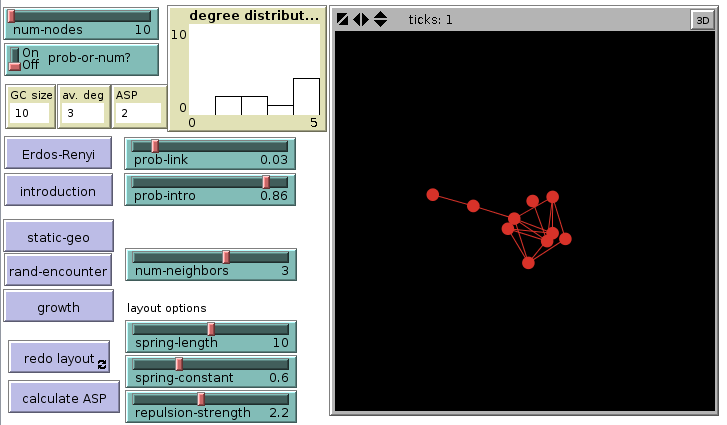
\includegraphics[width=0.5\textwidth]{er10}
            \label{er10}
        }
        \subfigure[Ejecución de una red de \textit{Erdös-Renyi} con 1000 nodos]{
            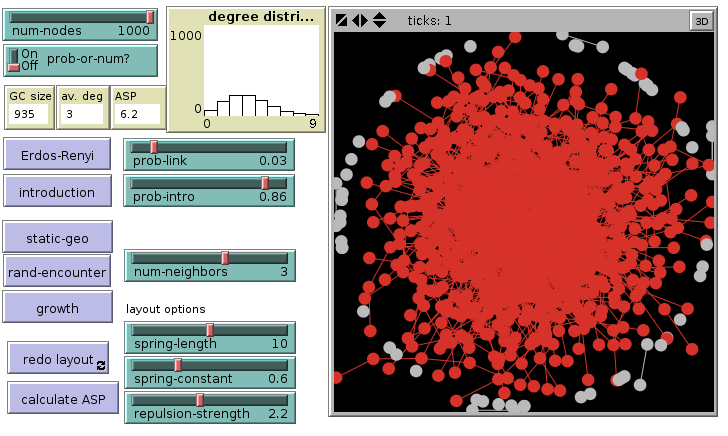
\includegraphics[width=0.5\textwidth]{er1000}
            \label{er1000}
        }
    }
    \caption{Comparación del camino medio más corto entre dos redes de \textit{Erdös-Renyi} con 10 y 1000 nodos respectivamente con el flag \texttt{prob-or-num?} desactivado.}
    \label{er}
\end{figure}

\begin{figure}[!h]
    \centering
    \mbox{
        \subfigure[Ejecución de una red de \textit{Erdös-Renyi} con 10 nodos y el flag \texttt{prob-or-num?} activado]{
            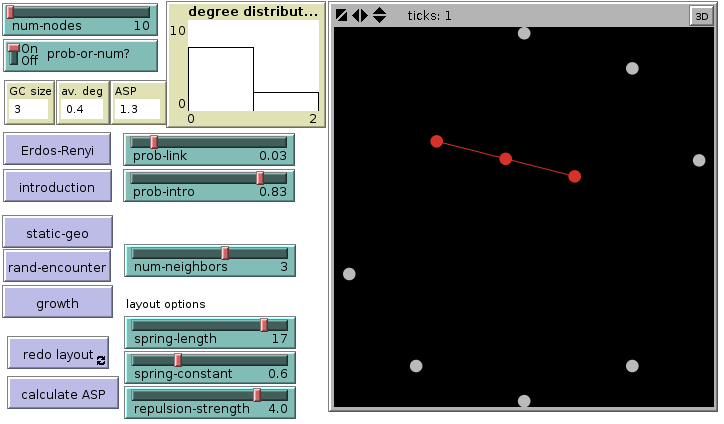
\includegraphics[width=0.5\textwidth]{er10on}
            \label{er10on}
        }
        \subfigure[Ejecución de una red de \textit{Erdös-Renyi} con 1000 nodos y el flag \texttt{prob-or-num?} activado]{
            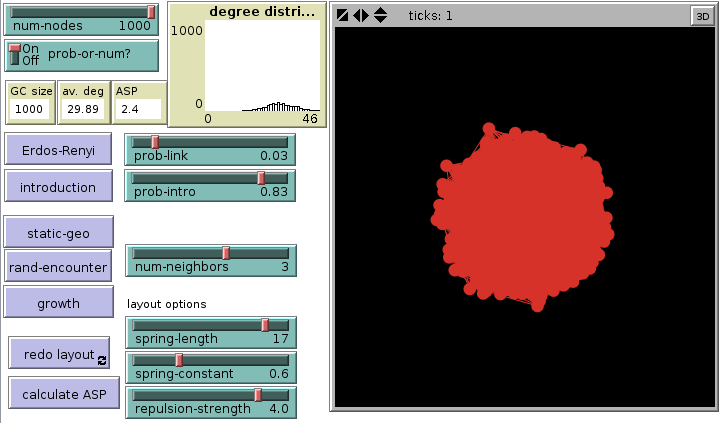
\includegraphics[width=0.5\textwidth]{er1000on}
            \label{er1000on}
        }
    }
    \caption{Comparación del camino medio más corto entre dos redes de \textit{Erdös-Renyi} con 10 y 1000 nodos respectivamente con el flag \texttt{prob-or-num?} activado.}
    \label{eron}
\end{figure}

}

\section{Modelo de Introducción}
\exe{En comparación con el modelo ER, el modelo de introducción 
\begin{enumerate}[\qquad a)]
    \item Tiene más enlaces.
    \item Tienes más cliques.
    \item Un camino mínimo medio más largo.
    \item Un grado más irregular.
    \item Una componente gigante más pequeña con valores bajos de $p$.
\end{enumerate}
}
\sol{En la \hyperref[cmpintrer]{Figura \ref*{cmpintrer}} comparamos una red ER con una de Introducción, hechas con los mismos parámetros. Las soluciones correctas son:

\begin{enumerate}[---]
    \item La \textbf{b} porque se ve claramente que \textbf{la red de Introducción tiene más cliques} que la ER.
    \item La \textbf{d} porque en las gráficas de distribución de grados, se ve que \textbf{la red ER tiene una distribución de grados más regular} que la red de introducción.
    \item La \textbf{e} porque con $p = 0.03$, \textbf{la componente gigante obtenida en la red ER es 4 veces mayor}.
\end{enumerate}

\begin{figure}[!h]
    \centering
    \mbox{
        \subfigure[Ejecución de una red de \textit{Erdös-Renyi} con 50 nodos]{
            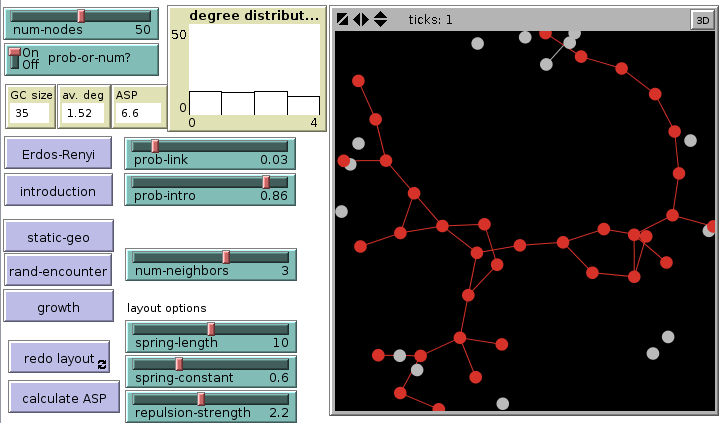
\includegraphics[width=0.5\textwidth]{er50}
            \label{er50}
        }
        \subfigure[Ejecución de una red de \textit{Introducción} con 50 nodos]{
            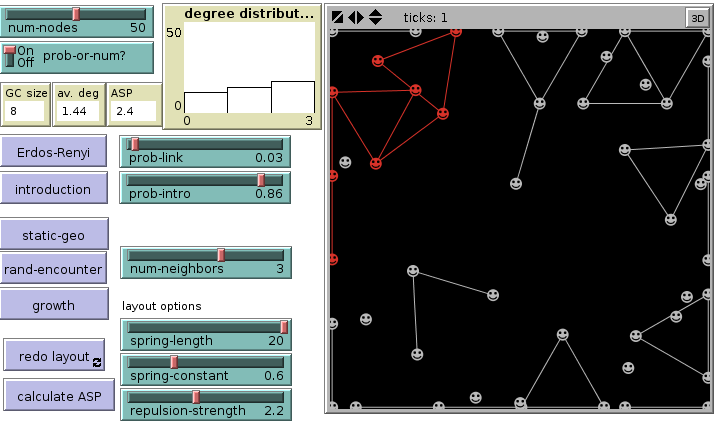
\includegraphics[width=0.5\textwidth]{intr50}
            \label{intr50}
        }
    }
    \caption{Comparación de una red \textit{Erös-Renyi} con una red de \textit{Introducción}}
    \label{cmpintrer}
\end{figure}
}

\section{Modelo Estático Geográfico}
\exe{En relación con el modelo ER, el modelo estático geográfico tiene:
\begin{enumerate}[a)]
    \item Un camino mínimo medio más largo.
    \item Un camino mínimo medio más corto.
    \item Una distribución de grados más acotada.
    \item Una distribución de grados más amplia.
    \item Una componente gigante más pequeña con menor número de vecinos.
    \item Una componente gigante más grande con menor número de vecinos.
\end{enumerate}
}
\sol{}

\section{Modelo de Encuentros Aleatorios}
\textit{En relación con el modelo ER, el modelo de encuentros aleatorios tiene:
\begin{enumerate}[a)]
    \item Un mayor número de triángulos.
    \item Un menor número de triángulos.
    \item Una componente gigante menor con un menor número de vecinos.
    \item Una componente gigante mayor con un menor número de vecinos.
\end{enumerate}
}
\sol{}

\section{Modelo de crecimiento}
\textit{En relación con el modelo ER, el modelo de crecimiento tiene:
\begin{enumerate}[a)]
    \item Más hubs.
    \item Menos hubs.
    \item Una componente gigante menor con un menor número de vecinos.
    \item Una componente gigante mayor con un menor número de vecinos.
\end{enumerate}
}
\sol{}

\end{document}
